%-----------------------------------------------------------------------------
% header
%-----------------------------------------------------------------------------
%-----------------------------------------------------------------------------
% general document control
%\documentclass[11pt,a4paper,notitlepage]{article}
%\documentclass[journal]{ieeetr}

% journal specifics
\documentclass{article}
\usepackage{smc2012} 
\usepackage{times}
\usepackage{ifpdf}
\usepackage[english]{babel}
\usepackage{cite}
%\usepackage{mathptmx} 

% section counter
%\setcounter{secnumdepth}{1} 

% localization
\usepackage[utf8x]{inputenc}
%\usepackage[brazil]{babel}
%\usepackage{abntex}


% glossary
%\usepackage{glossaries}
%\makeglossaries
%\input{glossario}

% bibliography
%\usepackage[colorlinks,citecolor=blue,urlcolor=brown]{hyperref}
%\usepackage[alf]{abntcite}
%\usepackage[square,comma]{natbib}
%\usepackage[fixlanguage]{babelbib}
%\selectbiblanguage{portugues}


% embellishment
\usepackage{amssymb,amsmath,amsfonts}
\usepackage{booktabs}
%\numberwithin{equation}{section}
%\usepackage{enumerate}
%\usepackage[top=2.5cm, bottom=2.5cm, left=2.5cm, right=2.5cm]{geometry}
%\usepackage{xspace}
%\usepackage{colortbl}
%\usepackage{caption}
%\usepackage{mathdots}
%\usepackage{fancyhdr}
\usepackage{enumitem}
\setlist{nolistsep}


% figures
%\usepackage{graphicx}
%\usepackage{epsfig}

% math
\usepackage{amsthm}


%\usepackage{epstopdf}
%\usepackage[figure,table]{hypcap}	% corrects the hyper-anchor of figures/tables

% todo
%\usepackage[bordercolor=white,backgroundcolor=yellow!30,linecolor=black,colorinlistoftodos]{todonotes}
%\newcommand{\lembrete}[1]{\todo[color=cyan!20,inline]{\ensuremath{\rhd} #1}}


% new commands
%\newcommand{\FFT}{\texttt{FFT}\xspace}
%\newtheorem{definicao}{Definição}
%\newtheorem{exemplo}{Exemplo}
%\newtheorem{problema}{Problema}
%\newtheorem{algoritmo}{Algoritmo}
%\newtheorem{sistema}{Sistema}
\newcommand{\jclass}[1]{\texttt{\textmd{#1}}}

% hiphenation
\hyphenation{a-mount}

\usepackage{listings}
\usepackage{color}

\definecolor{dkgreen}{rgb}{0,0.4,0}
\definecolor{gray}{rgb}{0.5,0.5,0.5}
\definecolor{mauve}{rgb}{0.58,0,0.82}
\definecolor{LightCyan}{rgb}{0.7,0.9,0.9}
 
\lstset{ %
  language=C,                % the language of the code
  basicstyle=\ttfamily\footnotesize,           % the size of the fonts that are used for the code
  %numbers=left,                   % where to put the line-numbers
  numberstyle=\tiny,%\color{gray},  % the style that is used for the line-numbers
  stepnumber=1,                   % the step between two line-numbers. If it's 1, each line 
                                  % will be numbered
  numbersep=5pt,                  % how far the line-numbers are from the code
  %backgroundcolor=\color{white},      % choose the background color. You must add \usepackage{color}
  showspaces=false,               % show spaces adding particular underscores
  showstringspaces=false,         % underline spaces within strings
  showtabs=false,                 % show tabs within strings adding particular underscores
  frame=single,                   % adds a frame around the code
  %rulecolor=\color{black},        % if not set, the frame-color may be changed on line-breaks within not-black text (e.g. commens (green here))
  tabsize=2,                      % sets default tabsize to 2 spaces
  captionpos=b,                   % sets the caption-position to bottom
  breaklines=false,                % sets automatic line breaking
  breakatwhitespace=false,        % sets if automatic breaks should only happen at whitespace
  title=\lstname,                   % show the filename of files included with \lstinputlisting;
                                  % also try caption instead of title
  %keywordstyle=\color{blue},          % keyword style
  %commentstyle=\color{dkgreen},       % comment style
  %stringstyle=\color{mauve},         % string literal style
  escapeinside={\%*}{*)},            % if you want to add a comment within your code
  morekeywords={*,...},               % if you want to add more keywords to the set
  %xleftmargin=1em,
}


\newcommand{\figura}[3]{
\begin{figure}[h]
\begin{center}
\includegraphics[width=#2\textwidth]{#1}
\caption{#3}
\label{fig:#1}
\end{center}
\end{figure}
}


%-----------------------------------------------------------------------------
% journal specific commands
%-----------------------------------------------------------------------------

%user defined variables
\def\papertitle{Real time digital audio processing using Arduino}
\def\firstauthor{André Jucovsky Bianchi}
\def\secondauthor{Marcelo Queiroz}
\def\thirdauthor{Third author}

%-----------------------------------------------------------------------------
% Dados do trabalho
%\title{}
%\author{André Jucovsky Bianchi \\
%\small{Departamento de Ciência da Computação \\
%Instituto de Matemática e Estatística \\
%Universidade de São Paulo \\
%\texttt{ajb@ime.usp.br}}}

\newif\ifpdf
\ifx\pdfoutput\relax
\else
   \ifcase\pdfoutput
      \pdffalse
   \else
      \pdftrue
\fi

\ifpdf % compiling with pdflatex
  \usepackage[pdftex,
    pdftitle={\papertitle},
    pdfauthor={\firstauthor, \secondauthor, \thirdauthor},
    bookmarksnumbered, % use section numbers with bookmarks
    pdfstartview=XYZ % start with zoom=100% instead of full screen; 
                     % especially useful if working with a big screen :-)
   ]{hyperref}
  %\pdfcompresslevel=9

  \usepackage[pdftex]{graphicx}
  % declare the path(s) where your graphic files are and their extensions so 
  %you won't have to specify these with every instance of \includegraphics
  \graphicspath{{./img/}}
  \DeclareGraphicsExtensions{.pdf,.jpeg,.png}

  \usepackage[figure,table]{hypcap}

  \usepackage{epstopdf}

\else % compiling with latex
  \usepackage[dvips,
    bookmarksnumbered, % use section numbers with bookmarks
    pdfstartview=XYZ % start with zoom=100% instead of full screen
  ]{hyperref}  % hyperrefs are active in the pdf file after conversion

  \usepackage[dvips]{epsfig,graphicx}
  % declare the path(s) where your graphic files are and their extensions so 
  %you won't have to specify these with every instance of \includegraphics
  \graphicspath{{./img/}}
  \DeclareGraphicsExtensions{.eps}

  \usepackage[figure,table]{hypcap}
\fi

%setup the hyperref package - make the links black without a surrounding frame
\hypersetup{
    colorlinks,%
    citecolor=black,%
    filecolor=black,%
    linkcolor=black,%
    urlcolor=black
}

% Title.
% ------
\title{\papertitle}

% Authors
% Please note that submissions are NOT anonymous, therefore 
% authors' names have to be VISIBLE in your manuscript. 
%
% Single address
% To use with only one author or several with the same address
% ---------------
%\oneauthor
%   {\firstauthor} {Affiliation1 \\ %
%     {\tt \href{mailto:author1@smcnetwork.org}{author1@smcnetwork.org}}}

%Two addresses
%--------------
\twoauthors
  {\firstauthor} {Computer Science Department \\
                  University of São Paulo \\ %
    {\tt \href{mailto:ajb@ime.usp.br}{ajb@ime.usp.br}}}
  {\secondauthor} {Computer Science Department \\
                  University of São Paulo \\ %
    {\tt \href{mailto:mqz@ime.usp.br}{mqz@ime.usp.br}}}

% Three addresses
% --------------
% \threeauthors
%   {\firstauthor} {Affiliation1 \\ %
%     {\tt \href{mailto:author1@smcnetwork.org}{author1@smcnetwork.org}}}
%   {\secondauthor} {Affiliation2 \\ %
%     {\tt \href{mailto:author2@smcnetwork.org}{author2@smcnetwork.org}}}
%   {\thirdauthor} { Affiliation3 \\ %
%     {\tt \href{mailto:author3@smcnetwork.org}{author3@smcnetwork.org}}}

%-----------------------------------------------------------------------------
% Document
\begin{document}

%
\capstartfalse
\maketitle
\capstarttrue

%
% sumário
%\tableofcontents

\maketitle

\begin{abstract}

% contexto do trabalho
% problema que resolve
% por que é um problema interessante
% quais as consequências

In the search for low-cost, highly available devices for real time audio
processing for scientific or artistic purposes, the Arduino platform comes in
as a handy alternative as a chordless, versatile audio processor. Despite the
fact that Arduinos are generally used for controlling and interfacing with
other devices, its builtin ADC/DAC allows for capturing and emitting raw audio
signals with very specific constraints. In this work we dive into the
microcontroller's structure to understand what can be done and what are the
limits of the platform when working with real time digital signal processing.
We evaluate the behaviour of some common DSP algorithms and expose limitations
and possibilities of using the platform in this context.


\end{abstract}

%-----------------------------------------------------------------------------
%  ___       _                 _            _   _             
% |_ _|_ __ | |_ _ __ ___   __| |_   _  ___| |_(_) ___  _ __  
%  | || '_ \| __| '__/ _ \ / _` | | | |/ __| __| |/ _ \| '_ \ 
%  | || | | | |_| | | (_) | (_| | |_| | (__| |_| | (_) | | | |
% |___|_| |_|\__|_|  \___/ \__,_|\__,_|\___|\__|_|\___/|_| |_|
%-----------------------------------------------------------------------------

\section{Introduction}


Arduino is the name of a hardware and software project started in 2005 which
aims to simplify the interface of electric-electronic devices with a
microcontroller. It evolved from the Processing software IDE (2001) and the
Wiring software and hardware prototyping platform (2003). Hardware, software
and documentation designs are published under free licenses (Creative Commons
BY-SA 2.5, GPL/LGPL and CC BY-SA 3.0 respectively) and a large community has
grown to provide code and support for newcomers. Nowadays, many Arduino
hardware designs are available and range from more limited 8-bit
microcontrollers to fully featured 32-bit ARM CPUs. Besides, other
advantages of Arduino for academic and artistic use are its mobility (because
of its low power needs and possibility of running on batteries for hours, if
not days depending on the use), expandability (because of its standardized
interface for attaching so called hardware \emph{shields}) and price (selling
for under 20 US dollars online).

Despite all these advantages, the platform has a somewhat limited processing
power when compared to standard processors available in the market for
specific or general uses. In this work, we aim to systematically expose the
platform's possibilities for carrying real time digital audio processing tasks
so there can be more accurate elements to be taken into account when making
the choice for a platform.


\subsection{Related work}

Arduino has been experimentally used for real time audio processing for sampling audio and control signals with an effective rate of 15.250~KHz \cite{arduinodsp}, and provided the base for our investigation. Also, an ALSA audio driver was implemented to use the Arduino Duemillanove \cite{Dimitrov:2011} as a full-duplex, mono, 8-bit 44.1~KHz sound card under linux.

%\subsection{Text organization}


%-----------------------------------------------------------------------------
\section{DSP em Arduino}
%-----------------------------------------------------------------------------


\subsection{Entrada de áudio: ADC}

%-----------------------------------------------------------------------------
\begin{frame}{Conversor analógico-digital (ADC)}
Características do ADC no ATmega328P:
\begin{itemize}
  \item Amostragem:
    \begin{enumerate}
      \item \emph{Sample and hold}.
      \item Aproximação sucessiva.
    \end{enumerate}
  \item Resolução: 8 ou 10 bits.
  \item Tempo de conversão: 13 a 260 $\mu$s.
  \item Frequência própria / redução de ruído.
  \item Conversão manual ou automática.
\end{itemize}
\end{frame}
%-----------------------------------------------------------------------------

%-----------------------------------------------------------------------------
\begin{frame}{Conversor analógico-digital (ADC)}
Medição do tempo de conversão, usando diferentes valores de pré-escalonador
(frequência principal: 16~MHz):
\begin{center}
\begin{tabular}{crrrr}
\toprule
\toprule
\footnotesize{pré-escalonador} & \footnotesize{$f_\text{ADC}$ (KHz)} &
\footnotesize{$T_\text{ADC}$ ($\mu$s)} & \footnotesize{$\tilde{T}_\text{conv}$ ($\mu$s)} & \footnotesize{$\tilde{f}_\text{conv}$ ($\approx$Hz)} \\
\midrule
2 & 8.000 & 0,125 & 12,61 & 79.302\\
4 & 4.000 & 0,25 & 16,06  & 62.266 \\
\rowcolor{LightCyan}
8 & 2.000 & 0,50 & 19,76  & 50.607 \\
16& 1.000 & 1 & 20,52  & 48.732 \\
32& 500 & 2 & 34,80  & 28.735 \\
64& 250 & 3 & 67,89  & 14.729 \\
128& 125 & 8 & 114,85 & 8.707  \\
\bottomrule
\end{tabular}
\end{center}
Obs:
\begin{itemize}
  \item Resolução da função \texttt{micros()}: 4~$\mu$s.
  \item Período de conversão: $\approx$ $14,5 \times T_\text{ADC}$. 
  \item $R=44.100$~Hz $\Rightarrow$ $T_\text{amostra} \approx 22,67~\mu$s.
  \item $R=31.250$~Hz $\Rightarrow$ $T_\text{amostra} = 32,00~\mu$s.
\end{itemize}
\end{frame}
%-----------------------------------------------------------------------------

%-----------------------------------------------------------------------------
\begin{frame}{Conversor analógico-digital (ADC)}
Parâmetros escolhidos:
\begin{itemize}
  \item Conversão alinhada à esquerda (8 bits).
  \item Pré-escalonador igual a 8.
\end{itemize}
\end{frame}
%-----------------------------------------------------------------------------

\subsection{Saída de áudio: PWM}

%-----------------------------------------------------------------------------
\begin{frame}{Modulação por largura de pulso (PWM)}
\begin{figure}
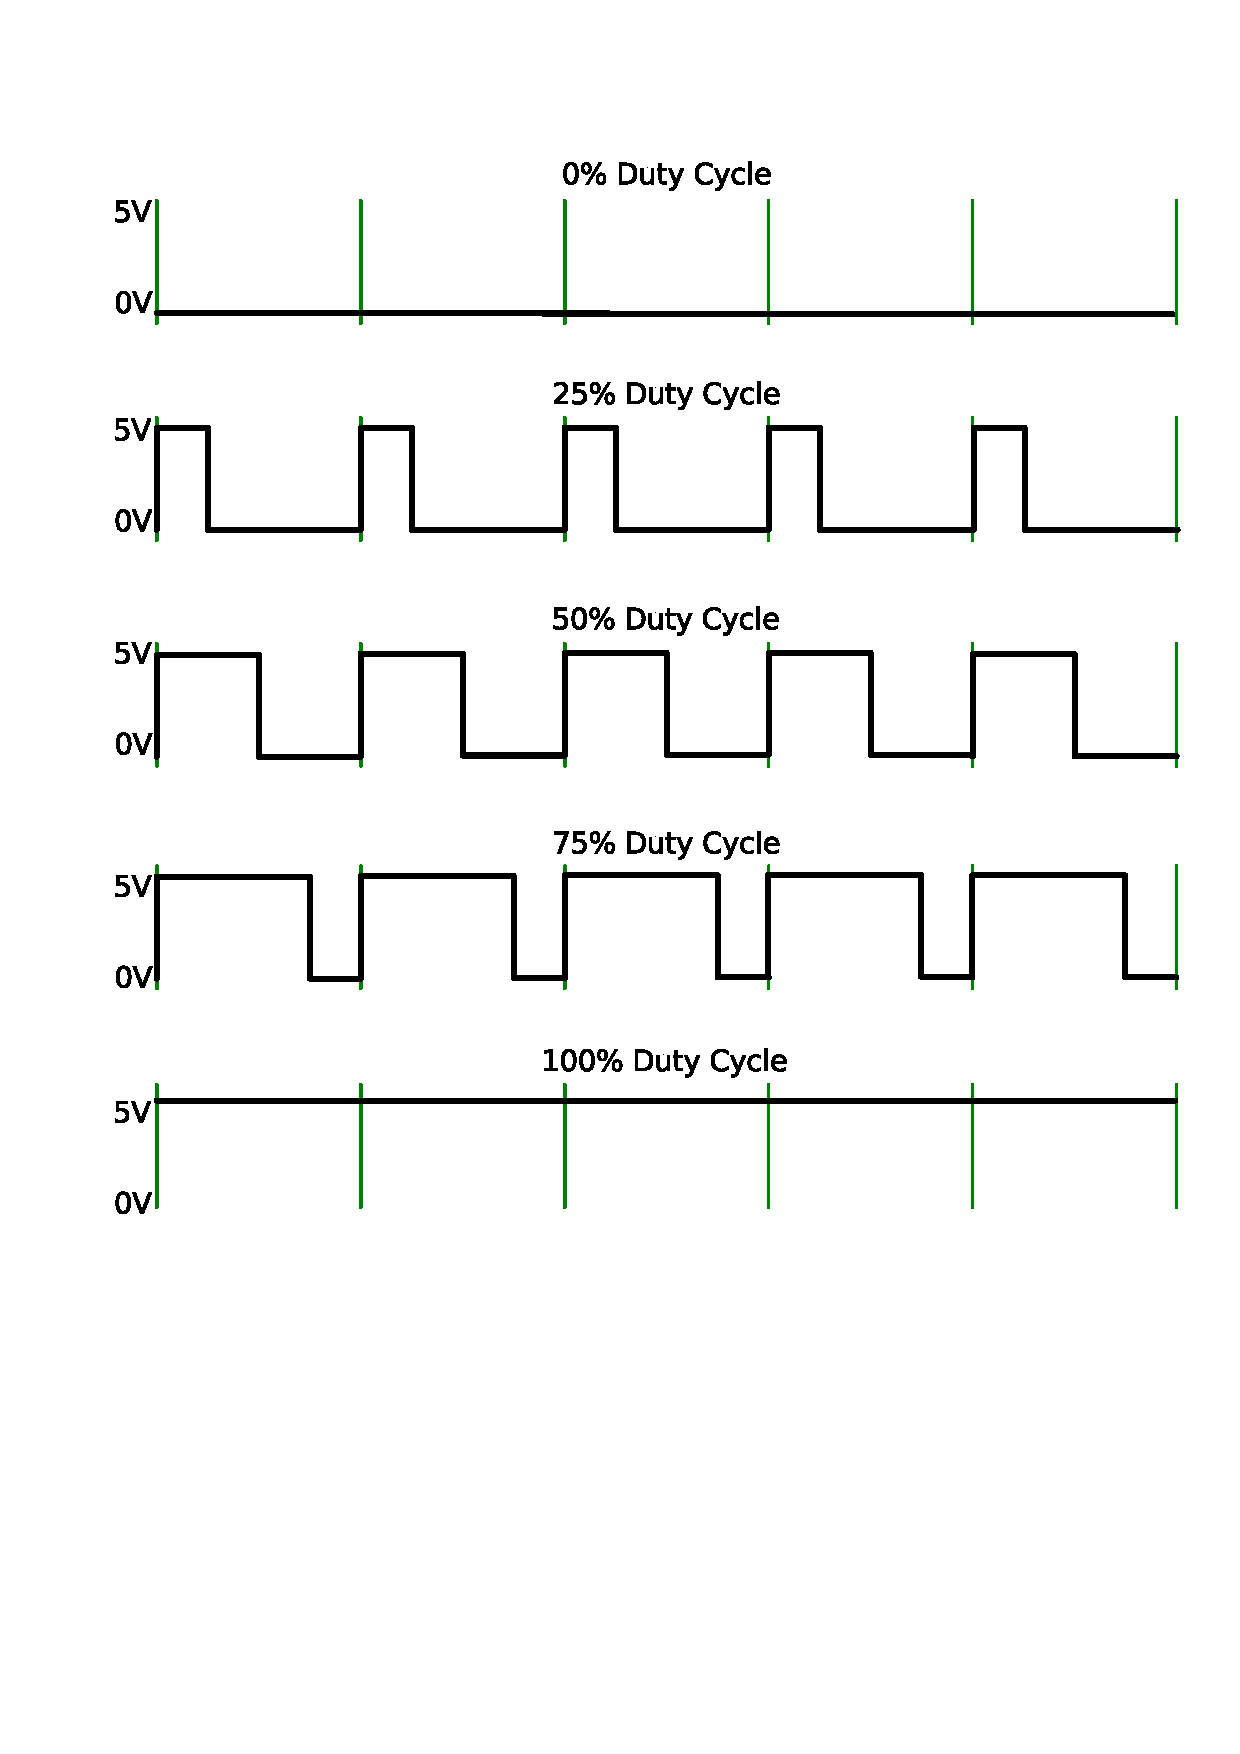
\includegraphics[height=0.8\textheight]{./img/pwmmeu.pdf}
\end{figure}
\end{frame}
%-----------------------------------------------------------------------------

%-----------------------------------------------------------------------------
\begin{frame}{Modulação por largura de pulso (PWM)}
\begin{figure}
\includegraphics[width=\textwidth]{./img/pwm2.pdf}
\end{figure}
\end{frame}
%-----------------------------------------------------------------------------

%-----------------------------------------------------------------------------
\begin{frame}{Modulação por largura de pulso (PWM)}
\begin{figure}
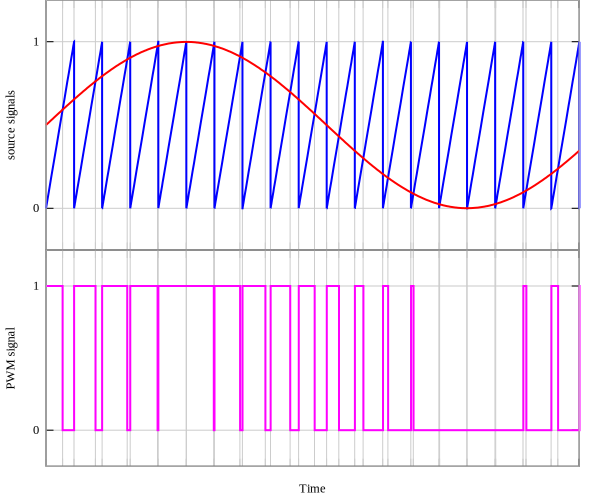
\includegraphics[width=0.8\textwidth]{./img/Pwm.pdf}
\end{figure}
\end{frame}
%-----------------------------------------------------------------------------

%-----------------------------------------------------------------------------
\begin{frame}{Modulação por largura de pulso (PWM)}
Características de PWM no ATmega328P:
\begin{itemize}
  \item 6 canais de saída.
  \item Modos de operação: \emph{Fast} e \emph{Phase Correct}.
  \item Pré-escalonador.
%  \item Compare Match output mode.
  \item 2 contadores de 8 bits e 1 de 16 bits.
%  \item Período fixo e variável.
  \item Interrupção por transbordamento.
\end{itemize}
\end{frame}
%-----------------------------------------------------------------------------

%-----------------------------------------------------------------------------
\begin{frame}{Modulação por largura de pulso (PWM)}
Frequências de operação de um contador de 8 bits:
\begin{center}
\begin{tabular}{crrrr}
\toprule
\toprule
\footnotesize{pré-escalonador} &
\footnotesize{$f_\text{incr}$ (KHz)} &
\footnotesize{$f_\text{overflow}$ (Hz)}  \\
\midrule
\rowcolor{LightCyan}
1 & 16.000 & 62.500 \\
8 & 2.000 & 7.812 \\
32 & 500 & 1.953 \\
64 & 250 & 976 \\
128 & 125 & 488 \\
256 & 62,5 & 244 \\
1024 & 15,625 & 61 \\
\bottomrule
\end{tabular}
\end{center}
\end{frame}
%-----------------------------------------------------------------------------

%-----------------------------------------------------------------------------
\begin{frame}{Modulação por largura de pulso (PWM)}
Parâmetros escolhidos:
\begin{itemize}
  \item \emph{Fast PWM}.
  \item Contador de 8 bits.
  \item Pré-escalonador igual a 1.
  \item Frequência de \emph{overflow}: 16~MHz / 1 / $2^8$ = 62.500~Hz.
  \item Taxa de geração de amostras: 31.250~Hz.
\end{itemize}
\end{frame}
%-----------------------------------------------------------------------------
\subsection{Processamento}


%-----------------------------------------------------------------------------
\begin{frame}[fragile]{Acoplamento de entrada e saída}
\begin{lstlisting}
// 1. leitura da entrada: ADC
x[ind] = ADCH;

// 2. escrita na saida: PWM
OCR2A = y[(ind-MIN_DELAY)&(BUFFER_SIZE-1)];

// 3. sinalizacao de um novo bloco de amostras
if ((ind & (BLOCK_SIZE - 1)) == 0) {
  rind = (ind-BLOCK_SIZE) & (BUFFER_SIZE-1);
  dsp_block = true;
}

// 4. incremento do indice de leitura/escrita
ind++;
ind &= BUFFER_SIZE - 1;

// 5. inicia uma nova conversao ADC
sbi(ADCSRA,ADSC); 
\end{lstlisting}
\end{frame}
%-----------------------------------------------------------------------------


%-----------------------------------------------------------------------------
\begin{frame}[fragile]{Implementação}
Detalhes importantes para implementar o sistema:
\begin{itemize}
  \item ADC:
  \begin{itemize}
    \item Valor do pré-escalonador.
    \item Alinhamento do resultado (resolução).
    \item Valor de referência.
    \item Pino de entrada.
  \end{itemize}
  \item PWM:
  \begin{itemize}
    \item Modo \emph{Fast PWM}.
    \item Valor do pré-escalonador.
    \item Pino de saída.
  \end{itemize}
  \item Compilação: \texttt{avr-gcc}, \texttt{avr-g++}.
  \item Monitoramento serial: \texttt{minicom}.
\end{itemize}
\end{frame}
%-----------------------------------------------------------------------------


%-----------------------------------------------------------------------------
\begin{frame}{Memória}
Limites da Memória:
\begin{itemize}
  \item 2~Kb de SRAM para dados.
  \item Uma tabela com 512 bytes ocupa $\frac{1}{4}$ da memória!
  \item Buffer máximo de 2.000 amostras.
\end{itemize}
\end{frame}
%-----------------------------------------------------------------------------




%-----------------------------------------------------------------------------
% ____                 _ _       
%|  _ \ ___  ___ _   _| | |_ ___ 
%| |_) / _ \/ __| | | | | __/ __|
%|  _ <  __/\__ \ |_| | | |_\__ \
%|_| \_\___||___/\__,_|_|\__|___/
%-----------------------------------------------------------------------------

\section{Results}
\label{sec:results}

%-----------------------------------------------------------------------------
%     _       _     _ _ _   _             ____              _   _     
%    / \   __| | __| (_) |_(_)_   _____  / ___| _   _ _ __ | |_| |__  
%   / _ \ / _` |/ _` | | __| \ \ / / _ \ \___ \| | | | '_ \| __| '_ \ 
%  / ___ \ (_| | (_| | | |_| |\ V /  __/  ___) | |_| | | | | |_| | | |
% /_/   \_\__,_|\__,_|_|\__|_| \_/ \___| |____/ \__, |_| |_|\__|_| |_|
%                                               |___/
%-----------------------------------------------------------------------------

\subsection{Additive synthesis}

\figura{./img/operations-128-31250.pdf}{0.35}{Type and number of operations
make a difference.}

\figura{./img/sinesum-comparison.pdf}{0.35}{Results for blocks of different
sizes.}

\figura{./img/sinesum-comparison-for.pdf}{0.35}{Results for blocks of different
sizes.}

\figura{./img/frequencies-128-1.pdf}{0.35}{Results for different sample rates.}

Result summary:

\begin{center}
\begin{tabular}{rcccc}
\toprule
\toprule
block size  & 2op & 1op & pad+for & pad \\
\midrule
32  & 2 & 4 & 8 & 14 \\
64  & 2 & 4 & 8 & 14 \\
128 & 2 & 4 & 8 & 15 \\
\bottomrule
\end{tabular}
\end{center}


%-----------------------------------------------------------------------------
%   ____                      _       _   _             
%  / ___|___  _ ____   _____ | |_   _| |_(_) ___  _ __  
% | |   / _ \| '_ \ \ / / _ \| | | | | __| |/ _ \| '_ \ 
% | |__| (_) | | | \ V / (_) | | |_| | |_| | (_) | | | |
%  \____\___/|_| |_|\_/ \___/|_|\__,_|\__|_|\___/|_| |_|
%                                                       
%-----------------------------------------------------------------------------

\figura{./img/convolution-comparison-cpad.pdf}{0.35}{TODO: change caption}

{Convolução no domínio do tempo}{Resultados para blocos de diferentes tamanhos}

\figura{./img/convolution-comparison-vpad.pdf}{0.35}{TODO: change caption}

\figura{./img/convolution-comparison-mult.pdf}{0.35}{TODO: change caption}

Ordem máxima do filtro FIR em cada cenário ($R=31.250$~Hz):

\begin{center}
\begin{tabular}{rccc}
\toprule
\toprule
\footnotesize{block size}  & \footnotesize{multiplicação} & \footnotesize{pad variável} & \footnotesize{pad constante} \\
\midrule
32  & 1 & 7 & 13 \\
64  & 1 & 7 & 13 \\
128 & 1 & 7 & 14 \\
256 & 1 & 7 & 14 \\
\bottomrule
\end{tabular}
\end{center}

%-----------------------------------------------------------------------------
{Exemplo: moving average}
\figura{./img/moving.pdf}{0.35}{TODO: change caption}


%-----------------------------------------------------------------------------
%  _____ _____ _____ 
% |  ___|  ___|_   _|
% | |_  | |_    | |  
% |  _| |  _|   | |  
% |_|   |_|     |_|  
%
%-----------------------------------------------------------------------------


\figura{./img/fft.pdf}{0.35}{TODO: change caption}

%-----------------------------------------------------------------------------
Determinação de frequência máxima:
\begin{itemize}
  \item Média de 428,15~$\mu$s por amostra.
  \item Frequência máxima $\approx$ 2.335~Hz.
  \item Pré-escalonador PWM de 32 $\Rightarrow$ $R=1.953$~Hz.
\end{itemize}
%-----------------------------------------------------------------------------

\figura{./img/fft2.pdf}{0.35}{TODO: change caption}



%-----------------------------------------------------------------------------
% ____  _                        _             
%|  _ \(_)___  ___ _   _ ___ ___(_) ___  _ __  
%| | | | / __|/ __| | | / __/ __| |/ _ \| '_ \ 
%| |_| | \__ \ (__| |_| \__ \__ \ | (_) | | | |
%|____/|_|___/\___|\__,_|___/___/_|\___/|_| |_|
%-----------------------------------------------------------------------------

\section{Discussion}
\label{sec:discussion}


\begin{itemize}
    \item The types used (byte, unsigned long, int, float, etc) are
    fundamental.
    \item Integer multiplication/division takes at least double time time than
    operations on integers only.
    \item The amount of loops make a difference.
    \item Consulting variables also makes a difference.
\end{itemize}



\subsection{Future work}



\section{Acknowledgements}

We would like to thank the members of the Computer Music
Group\footnote{http://compmus.ime.usp.br/en/} of the Computer Science
Department of the Institute of Mathematics and Statistics of the University of
São Paulo. This work has been supported by the funding agencies CAPES and
FAPESP (grant 2008/08632-8).

%-----------------------------------------------------------------------------
% Glossário
%\printglossaries

% Bibliografia
%\bibliographystyle{abnt-alf}
\nocite{*}
%\bibliographystyle{IEEEtranS}
%\bibliographystyle{plain}
%\bibliography{references}

\end{document}
